\documentclass[10pt,a4paper]{article}
\usepackage[latin1]{inputenc}
\usepackage{amsmath}
\usepackage{amsfonts}
\usepackage{amssymb}
\usepackage{float}
\usepackage{graphicx}
\begin{document}
\section{Descripci�n del problema.}
El objetivo de esta competici�n es predecir de la forma m�s exacta posible el precio de las casas residenciales en Ames, Iowa, a partir de 79 variables explicativas que describen casi todos los aspectos.
\subsection{Variables}
	\begin{itemize}
		\item SalePrice - the property's sale price in dollars. This is the target variable that you're trying to predict.
		\item MSSubClass: The building class
		\item MSZoning: The general zoning classification
		\item LotFrontage: Linear feet of street connected to property
		\item LotArea: Lot size in square feet
		\item Street: Type of road access
		\item Alley: Type of alley access
		\item LotShape: General shape of property
		\item LandContour: Flatness of the property
		\item Utilities: Type of utilities available
		\item LotConfig: Lot configuration
		\item LandSlope: Slope of property
		\item Neighborhood: Physical locations within Ames city limits
		\item Condition1: Proximity to main road or railroad
		\item Condition2: Proximity to main road or railroad (if a second is present)
		\item BldgType: Type of dwelling
		\item HouseStyle: Style of dwelling
		\item OverallQual: Overall material and finish quality
		\item OverallCond: Overall condition rating
		\item YearBuilt: Original construction date
		\item YearRemodAdd: Remodel date
		\item RoofStyle: Type of roof
		\item RoofMatl: Roof material
		\item Exterior1st: Exterior covering on house
		\item Exterior2nd: Exterior covering on house (if more than one material)
		\item MasVnrType: Masonry veneer type
		\item MasVnrArea: Masonry veneer area in square feet
		\item ExterQual: Exterior material quality
		\item ExterCond: Present condition of the material on the exterior
		\item Foundation: Type of foundation
		\item BsmtQual: Height of the basement
		\item BsmtCond: General condition of the basement
		\item BsmtExposure: Walkout or garden level basement walls
		\item BsmtFinType1: Quality of basement finished area
		\item BsmtFinSF1: Type 1 finished square feet
		\item BsmtFinType2: Quality of second finished area (if present)
		\item BsmtFinSF2: Type 2 finished square feet
		\item BsmtUnfSF: Unfinished square feet of basement area
		\item TotalBsmtSF: Total square feet of basement area
		\item Heating: Type of heating
		\item HeatingQC: Heating quality and condition
		\item CentralAir: Central air conditioning
		\item Electrical: Electrical system
		\item 1stFlrSF: First Floor square feet
		\item 2ndFlrSF: Second floor square feet
		\item LowQualFinSF: Low quality finished square feet (all floors)
		\item GrLivArea: Above grade (ground) living area square feet
		\item BsmtFullBath: Basement full bathrooms
		\item BsmtHalfBath: Basement half bathrooms
		\item FullBath: Full bathrooms above grade
		\item HalfBath: Half baths above grade
		\item Bedroom: Number of bedrooms above basement level
		\item Kitchen: Number of kitchens
		\item KitchenQual: Kitchen quality
		\item TotRmsAbvGrd: Total rooms above grade (does not include bathrooms)
		\item Functional: Home functionality rating
		\item Fireplaces: Number of fireplaces
		\item FireplaceQu: Fireplace quality
		\item GarageType: Garage location
		\item GarageYrBlt: Year garage was built
		\item GarageFinish: Interior finish of the garage
		\item GarageCars: Size of garage in car capacity
		\item GarageArea: Size of garage in square feet
		\item GarageQual: Garage quality
		\item GarageCond: Garage condition
		\item PavedDrive: Paved driveway
		\item WoodDeckSF: Wood deck area in square feet
		\item OpenPorchSF: Open porch area in square feet
		\item EnclosedPorch: Enclosed porch area in square feet
		\item 3SsnPorch: Three season porch area in square feet
		\item ScreenPorch: Screen porch area in square feet
		\item PoolArea: Pool area in square feet
		\item PoolQC: Pool quality
		\item Fence: Fence quality
		\item MiscFeature: Miscellaneous feature not covered in other categories
		\item MiscVal: \$Value of miscellaneous feature
		\item MoSold: Month Sold
		\item YrSold: Year Sold
		\item SaleType: Type of sale
		\item SaleCondition: Condition of sale
		
	\end{itemize}
\subsection{Evaluaci�n}
Teoria error logaritmico.
\section{Marco te�rico regresi�n.}
\section{Algoritmos.}
\textbf{Nota: Para la ejecuci�n de los algoritmos los datos nominales se han pasado a num�rico}

A priori desconocemos que algoritmo se adapta mejor a nuestro problema, es por ello que realizaremos un estudio comparando varios algoritmos. Los algoritmos elegidos son los siguientes:
\begin{itemize}
	\item Un algoritmo cl�sico como la regresi�n lineal.
	\item algoritmos "b�sicos" como KNN y Arboles de regresi�n
	\item algoritmos "potentes" como NeuralNetwork,Gaussian y SVM
	\item Multiclasificadores ya que debido a su f�cil paralelizaci�n ofrecen una buena escalabilidad. En este caso he seleccionado 3 algoritmos:
	\begin{itemize}
		\item Random Forest. Basado en crear muchos �rboles ligeramente diferentes y obtiene el resultado mediante el voto mayoritario.
		\item Boosting. Los �rboles se crean de forma lineal teniendo en cuenta los fallos anteriores. Esta t�cnica permite reducir el sesgo.
		\item Bagging.
	\end{itemize}
\end{itemize} En la siguiente gr�fica se muestran los resultados obtenidos.
\begin{figure}[H]
	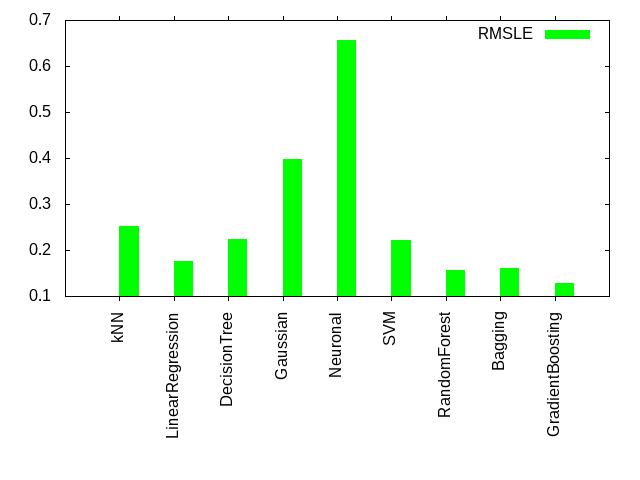
\includegraphics[scale=0.75]{./img/error.png}
	\caption{Test de algoritmos.Error.}
\end{figure}
Se puede observar que los algoritmos que mayor precisi�n proporcionan en este caso son los multiclasificadores. Por tanto, estudiaremos en profundidad RandomForest y Boosting para mejorar los resultados.
%En kaggle se suben 2 propuestas. 
\section{Herramientas.}
Otra decisi�n que debemos de tomar es qu� herramientas usar para abordar la resoluci�n del problema. Tras un estudio de las bibliotecas disponibles para los distintos lenguajes de programaci�n que domino, seleccion� weka(java), sklearn(python) y R. Para determinar cual de las 3 es la m�s conveniente en este caso, realizar� pruebas con los diferentes algoritmos y compararemos el tiempo de ejecuci�n y el uso de memoria. Adem�s, se debe tener en cuenta la facilidad para tratar los datos tanto para su lectura, como para la generaci�n de los archivos con las predicciones. 

Los resultados obtenidos se muestran en las siguientes gr�ficas:	
\begin{figure}[!h]
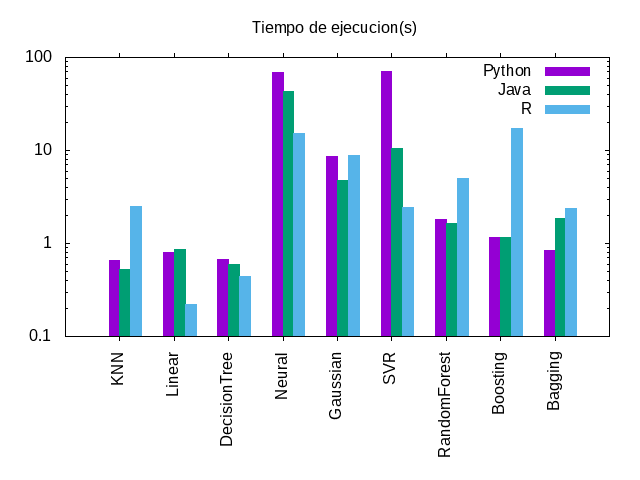
\includegraphics[scale=0.75]{./img/tiempos.png}
\caption{Test de algoritmos.Tiempo de ejecuci�n}
\end{figure}
\begin{figure}[H]
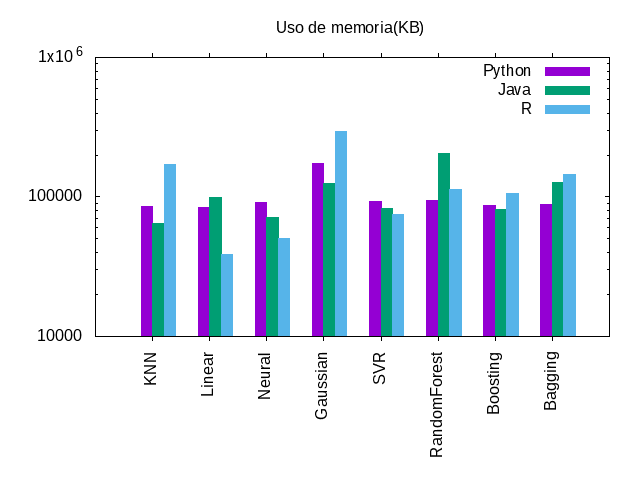
\includegraphics[scale=0.75]{./img/memoria.png}
\caption{Test de algoritmos.Memoria usada}
\end{figure}

Observando los resultados podemos concluir que sklearn y weka ofrecen (en media) un rendimiento similar, mientras que R ofrece un mayor rendimiento para los algoritmos b�sicos pero es inferior en la ejecuci�n de multiclasificadores.
Por otro lado, R y sklearn permiten tratar los datos de forma c�moda. Otra cuesti�n a tener en cuenta, es la buena documentaci�n con la que cuenta sklearn. 
%%sklearn proporciona el error logaritmico 

En conclusi�n, el lenguaje a usar ser� Python ya que permite un manejo de los datos flexible y un c�digo legible propio de este lenguaje. Esta decisi�n se apoya en que en t�rminos de rendimiento no hay una alternativa "mucho mejor". 

\section{Preprocesamiento.}
\end{document}